%%%%%%%%%%%%%%%%%%%%%%%%%%%%%%%%%%%%%%%%%%%%%%%%%%%%%%%%%%%%%%%%%%%%%%%%%%%%%%%
%
% Tommy P. Keane
% Master of Science Thesis
% Department of Electrical and Microelectronic Engineering
%
% March 2011
%
%
%
% .tex and .sty modified from:
% http://www.ce.rit.edu/studentresources/gradresource/LaTexThesis.zip
%
%%%%%%%%%%%%%%%%%%%%%%%%%%%%%%%%%%%%%%%%%%%%%%%%%%%%%%%%%%%%%%%%%%%%%%%%%%%%%%%

%%%%%%%%%%%%%%%%%%%%%%%%%%%%%%%%%%%%%%%%%%%%%%%%%%%%%%%%%%%%%%%%%%%%%%%%%%%%%%%
%
% CHAPTER 5
%
% SECTION 1
%
%%%%%%%%%%%%%%%%%%%%%%%%%%%%%%%%%%%%%%%%%%%%%%%%%%%%%%%%%%%%%%%%%%%%%%%%%%%%%%%


%%%%%%%%%%%%%%%%%%%%%%%%%%%%%%%%%%%%%%%%%%%%%%%%%%%%%%%%%%%%%%%%%%%%%%%%%%%%%%%
% BEGIN DOCUMENT

The rooftop scene, Figure \ref{RooftopImages}, is a view from the Tufts University campus in Massachussetts. As mentioned, this is a large image that has been cropped into two overlapping views. By testing the WFMI algorithm with these two ideal views (and other similar scenarios) a better understanding of the feature generation, entropy concerns, and overlap limitations for the algorithm were found. Through empirical testing of affine views of realistic (but affine) scenes it was found that a minimum of 10\% pixel overlap could be tolerated on average. As the entropy of  the scene in the overlap region increases, more distinct and varied features can be generated, and the less overlap that is required between the views. This directly follows from the implementation of the WFMI metric which calculates similarity based on the distributions of features in the overlap regions. Scenes with large amounts of entropy will have very distinct features that will have a low probability of re-occuring elsewhere in the scene, and thus elsewhere in any of the views besides in the overlapping view. In an extremely unrealistic, high entropy, case it was found that the WFMI algorithm can register views with only 1\% of the total pixels overlapping. To provide a general metric, realistic affine views of a purely affine scene were found to require a minimum of 10-15\% of the total number of pixels be in the overlap region.

% ROOFTOP
\begin{figure}[!h]
\label{RooftopImages}
\centering
\subfigure{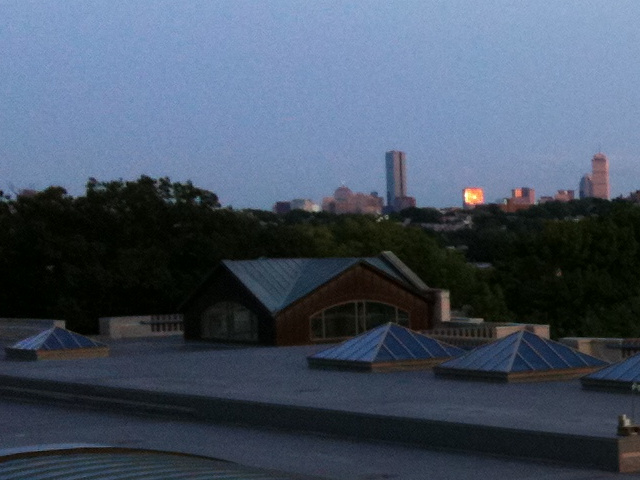
\includegraphics[width=.45\textwidth]{RooftopL001} \label{RooftopL}}
\subfigure{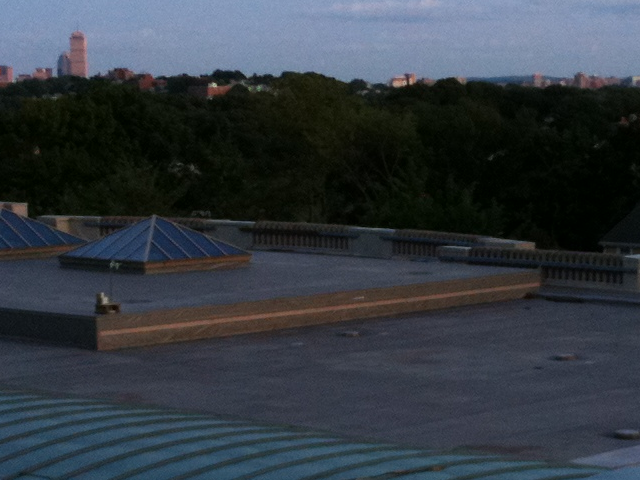
\includegraphics[width=.45\textwidth]{RooftopR001} \label{RooftopR}}
\caption{Rooftop Scene (a) Left View, (b) Right View}
\end{figure}

\begin{figure}[!h]
\centering
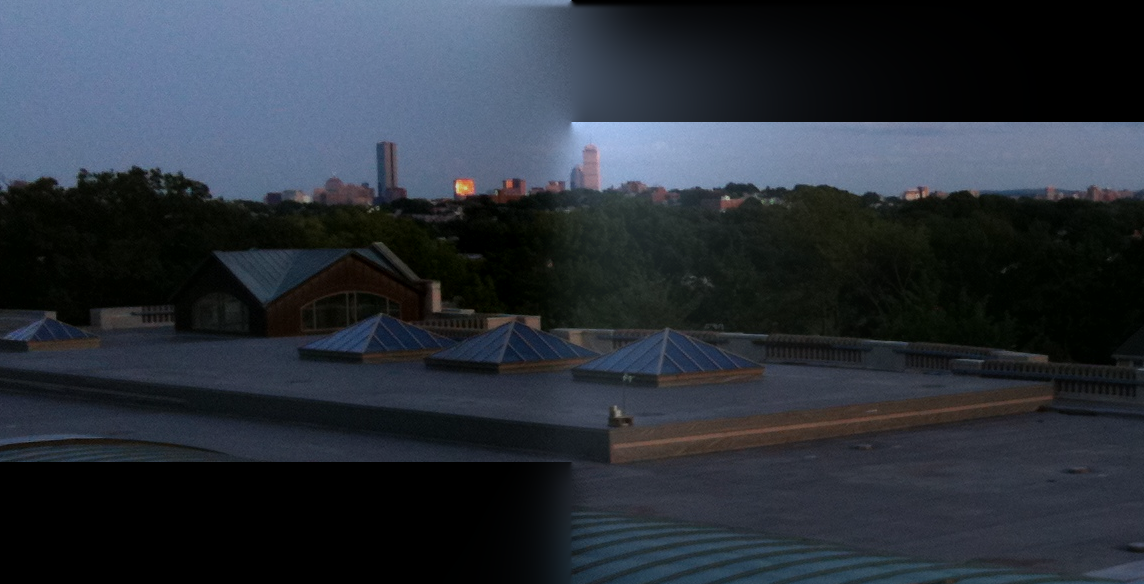
\includegraphics[width=1\textwidth]{RooftopSP001001}
\caption{Rooftop Views Blended}
\label{RooftopStitched}
\end{figure}

The automatically blended rooftop views in Figure \ref{RooftopStitched} can be compared to the manually blended views in Figure \ref{RooftopStitchedManual}. The manual blending technique follows the WFMI algorithm's mutli-resolution spline blending algorithm but the affine homography is generated by MATLAB\textsuperscript{\textregistered}'s feature correspondence selection tool (\textit{cpselect}) and the correspondence to transform function (\textit{cp2tform}).

\begin{figure}[!h]
\centering
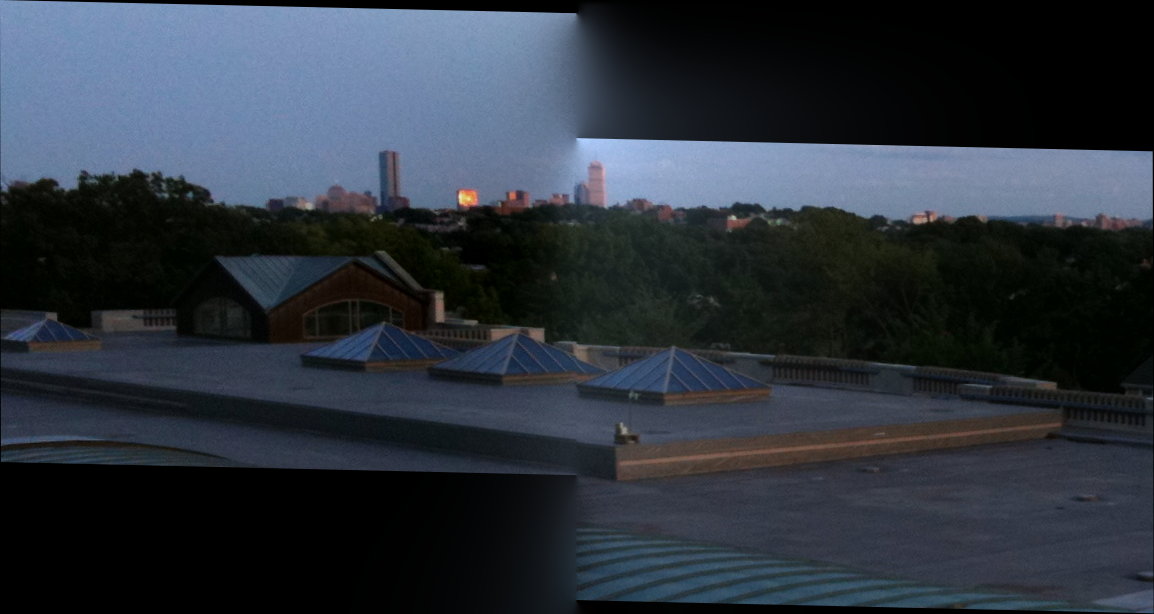
\includegraphics[width=1\textwidth]{RooftopSP001ManAff}
\caption{Rooftop Views Blended Manually (Affine)}
\label{RooftopStitchedManual}
\end{figure}

As can be seen in Figure \ref{RooftopStitchedManual} there is a rotation disparity from the manual results and the stitching seam is clearly visible as the views have been misregistered. In order to attempt to compare the algorithm to the manual method in terms of practical implementation, the feature points for the manual transform derivation were chosen relatively quickly at building and window corners. There were 12 to 15 points chosen and they automatically passed into the least-squared algorithm in MATLAB\textsuperscript{\textregistered}'s \textit{cp2tform} function.

An alternate affine set of views is presented in the stone wall scene. This is again a single view of a realistic scene with two overlapping affine views cropped from the larger view. This is a view of a wall and warehouse in Allston, MA. These views have only 5\% of the total image pixels in the overlap and are registered perfectly by the automatic WFMI algorithm.

% STONE WALL
\begin{figure}[!h]
\label{StoneWallImages}
\centering
\subfigure{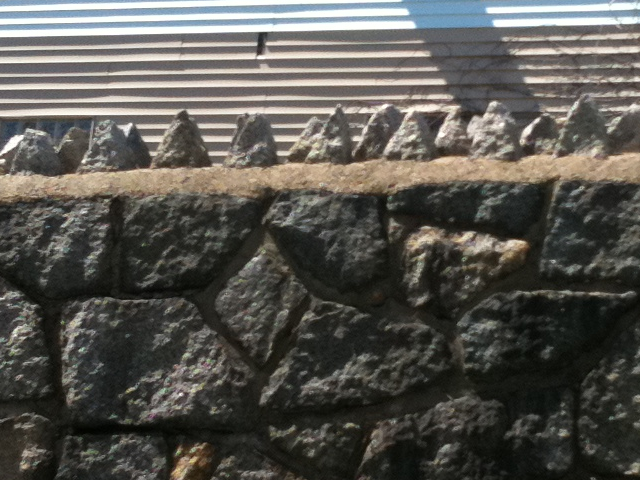
\includegraphics[width=.45\textwidth]{StoneWallL001} \label{StoneWallL}}
\subfigure{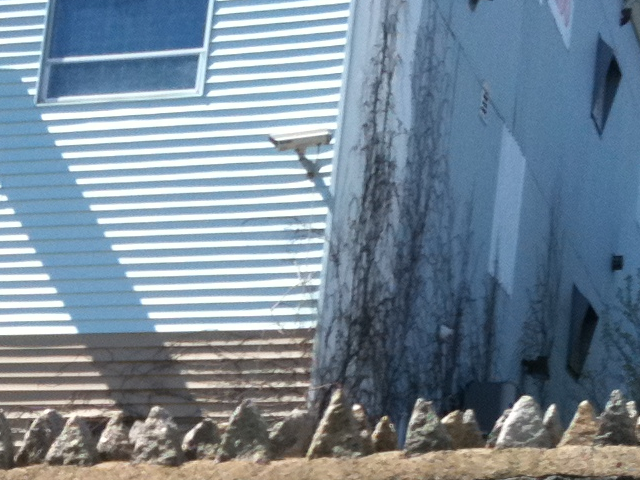
\includegraphics[width=.45\textwidth]{StoneWallR001} \label{StoneWallR}}
\caption{Stone Wall Scene (a) Left View, (b) Right View}
\end{figure}

\begin{figure}[!h]
\label{StoneWallStitched}
\centering
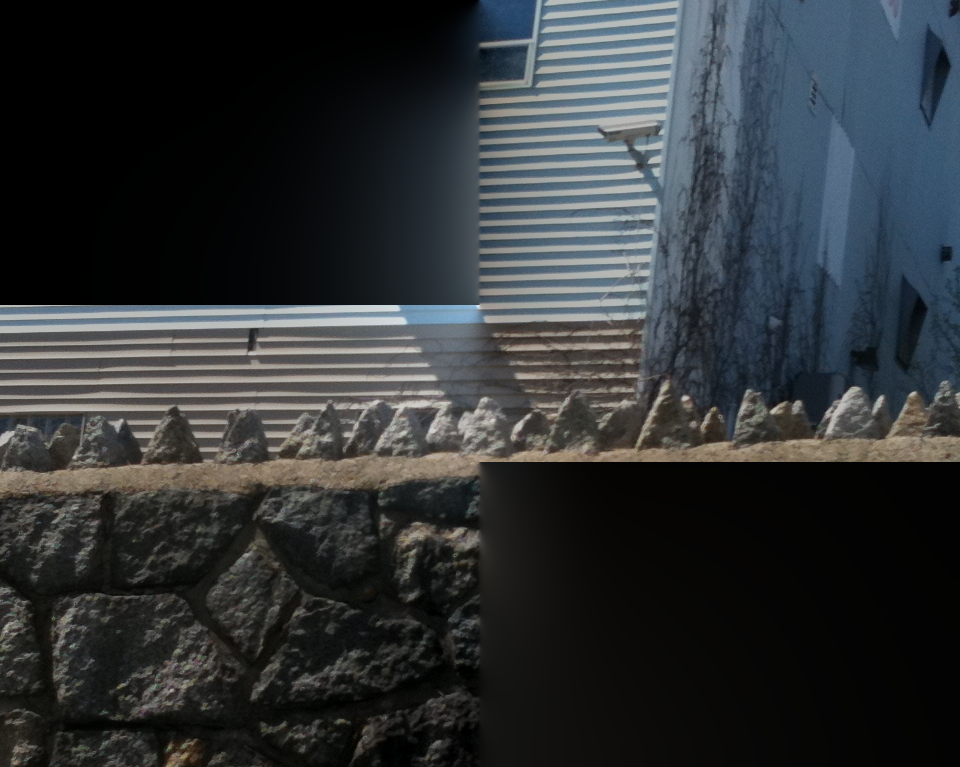
\includegraphics[width=1\textwidth]{StoneWallSP001001}
\caption{Stone Wall Views Blended}
\end{figure}



%%%%%%%%%%%%%%%%%%%%%%%%%%%%%%%%%%%%%%%%%%%%%%%%%%%%%%%%%%%%%%%%%%%%%%%%%%%%%%%
% END OF DOCUMENT
